% !TEX root = saveliev_physics_general_course_1.tex
%!TEX TS-program = pdflatex
%!TEX encoding = UTF-8 Unicode


\chapter{GENERAL INFORMATION}\label{chap:10}

\section{Statistical Physics and Thermodynamics}\label{sec:10_1}

Molecular physics is a branch of physics studying the structure and properties of a substance on the basis of the so-called molecular kinetic notions. According to these notions, any body-solid, liquid, or gaseous---consists of an enormous number of exceedingly small separate particles---molecules. (Atoms can be considered as monatomic molecules.) The molecules of a substance are in disordered, chaotic motion having no predominating direction. Its intensity depends on the temperature of the substance.

A direct proof of the existence of chaotic motion of molecules is Brownian motion. This phenomenon consists in that very small (visible only in a microscope) particles suspended in a fluid are always in a state of continuous chaotic motion that does not depend on external causes and is a manifestation of the internal motion of the substance. The Brownian motion of particles is due to their chaotic collisions with molecules.

The object of the molecular-kinetic theory is to interpret the properties of bodies that are directly observed in experiments (pressure, temperature, etc.) as the summary result of the action of molecules. It uses the statistical method and is interested not in the motion of separate molecules, but only in average quantities characterizing the motion of an enormous combination of particles. This explains its other name---statistical physics.

Thermodynamics also studies various properties of bodies and changes in the state of a substance. Unlike the molecular-kinetic theory, however, thermodynamics studies macroscopic properties of bodies and natural phenomena without being interested in their microscopic picture. Thermodynamics permits us to arrive at a considerable number of conclusions on how processes go on without taking molecules and atoms into consideration and without treating the processes from a microscopic standpoint.

Thermodynamics is founded on several fundamental laws established as a result of generalizing a large amount of experimental facts. Consequently, the conclusions of thermodynamics have a very general nature.

By considering the changes in the state of a substance from different viewpoints, thermodynamics and the molecular-kinetic theory mutually supplement each other, forming in essence a single entirety.

Turning to the history of the development of molecular-kinetic notions, we must point out first of all that ideas on the atomistic structure of a substance were already advanced by the ancient Greeks. These ideas, however, were nothing more than a brilliant conjecture. In the 17th century, atomistics again came to the forefront, but as a scientific hypothesis instead of a conjecture. This hypothesis was developed especially greatly in the works of the outstanding Russian scientist Mikhail Lomonosov (1711-1765). He attempted to give a single picture of all the physical and chemical phenomena known at his time. He proceeded from the corpuscular (according to modern terminology---molecular) notion of the structure of matter. Revolting against the theory of thermogen (a hypothetic thermal liquid whose content in a body determines the extent of its heating) that prevailed at his time, Lomonosov saw the ``cause of heat'' in the rotation of the particles of a body. Thus, Lomonosov in essence formulated molecular-kinetic ideas.

In the second half of the 19th century and at the beginning of the 20th century, atomistics became a scientific theory owing to the works of a number of scientists.

\section{Mass and Size of Molecules}\label{sec:10_2}

The masses of atoms and molecules are characterized by using quantities known as the \textbf{relative atomic mass of an element} (the atomic mass in short) and the \textbf{relative molecular mass of a substance} (the molecular mass). (These quantities were previously called the atomic weight and the molecular weight, respectively).

The atomic mass ($\amr$) of a chemical element is defined as the ratio of the mass of an atom of the element to $1/12$ of the mass of the atom \ce{C^12} (this is the symbol for the carbon isotope with a mass number of \num{12}). The molecular mass ($\mmr$) of a substance is defined as the ratio of the mass of a molecule of the substance to $1/12$ of the mass of the atom \ce{C^12}. Their definitions show that the atomic and molecular masses are dimensionless quantities.

A unit of mass equal to $1/12$ of the mass of the atom \ce{C^12} is called the \textbf{atomic mass unit} (\textbf{\si{\atomicmassunit}}). Let us denote the value of this unit expressed in kilogrammes by the symbol $\amu$. Hence, the mass of an atom expressed in kilogrammes will be $\amr\amu$, and the mass of a molecule will be $\mmr\amu$.

The amount of a substance containing a number of particles (atoms, molecules, ions, electrons, etc.) equal to the number of atoms in \SI{0.012}{\kilo\gram} of the carbon isotope \ce{C^12} is called a \textbf{mole} (the mole is a basic unit of the SI system). Multiple and submultiple units are also used such as the kilomole (\si{\kilo\mole}), the millimole (\si{\milli\mole}) and the micromole (\si{\micro\mole}).

The number of particles contained in a mole of a substance is called the \textbf{Avogadro constant}. It was found experimentally that the Avogadro constant is
\begin{equation}\label{eq:10_1}
	N_{\text{A}} = \SI{6.023e23}{\per\mole}.
\end{equation}

\noindent
Thus, for example, a mole of copper contains $N_{\text{A}}$ atoms of copper, a mole of water contains $N_{\text{A}}$ molecules of water, a mole of electrons contains $N_{\text{A}}$ electrons, etc.

The mass of a mole is called the molar mass $M$. It is evident that $M$ equals the product of $N_{\text{A}}$ and the mass of a molecule $\mmr\amu$:
\begin{equation}\label{eq:10_2}
	M = N_{\text{A}}\mmr\amu.
\end{equation}

For carbon \ce{C^12}, we have $M=\SI{0.012}{\kilo\gram\per\mole}$, and the mass of an atom is $12\amu$. Substitution of these values in \eqn{10_2} yields
\begin{equation*}
	\SI{0.012}{[\kilo\gram\per\mole]} = N_{\text{A}} [\si{\per\mole}] \times 12\amu [\si{\kilo\gram}].
\end{equation*}

\noindent
Hence,
\begin{align}
	\amu [\si{\kilo\gram}] &= \frac{\SI{0.001}{[\kilo\gram\per\mole]}}{N_{\text{A}} [\si{\per\mole}]} = \frac{0.001}{\num{6.023e23}}\nonumber\\
	&= \SI{1.66e-27}{\kilo\gram} = \SI{1.66e-24}{\gram}.\label{eq:10_3}
\end{align}

\noindent
Hence, the mass of any atom is $\num{1.66e-27}\amr\si{\kilo\gram}$, and the mass of any molecule is $\num{1.66e-27}\mmr\si{\kilo\gram}$.

It can be seen from \eqn{10_3} that the product $N_{\text{A}}\amu$ equals \SI{0.001}{\kilo\gram\per\mole}. Introducing this value in \eqn{10_2} we find that
\begin{equation}\label{eq:10_4}
	M = 0.001 \mmr\, \si{\kilo\gram\per\mole}
\end{equation}

\noindent
or
\begin{equation}\label{eq:10_5}
	M = \mmr\, \si{\gram\per\mole}.
\end{equation}

\noindent
Thus, the mass of a mole expressed in grammes numerically equals the relative molecular mass. It must be borne in mind, however, that whereas $\mmr$ is a dimensionless quantity, $M$ has a dimension and is measured in \si{\kilo\gram\per\mole} (or \si{\gram\per\mole}).

Now let us assess the size of molecules. It is natural to assume that molecules in a liquid are quite close to one another. We can therefore approximately find the volume of one molecule by dividing the volume of a mole of a liquid, for example, water, by the number of molecules in a mole $N_{\text{A}}$. One mole (\ie, \SI{18}{\gram}) of water occupies a volume of $\SI{18}{\centi\metre\cubed}=\SI{18e-6}{\metre\cubed}$. Hence, the volume falling to one molecule is
\begin{equation*}
	\frac{\num{18e-6}}{\num{6e23}} = \SI{30e-30}{\metre\cubed}.
\end{equation*}

\noindent
It follows that the linear dimensions of water molecules are approximately
\begin{equation*}
	\left(\num{30e-30}\right)^{1/3} \approx \SI{3e-10}{\metre} = \SI{3}{\angstrom}.
\end{equation*}

The molecules of other substances also have dimensions of the order of a few angstroms. (The angstrom---\si{\angstrom}--- is a non-system unit of length equal to \SI{e-10}{\metre}. It is very convenient in atomic physics.)

\section{State of a System. Process}\label{sec:10_3}

We shall call a combination of bodies being considered a \textbf{system of bodies} or simply a \textbf{system}. An example of a system is a liquid and the vapour in equilibrium with it. Particularly, a system may consist of one body.

Any system can be in different states distinguished by their temperature, pressure, volume, etc. Such quantities characterizing the state of a system are called \textbf{parameters} of state.

A parameter does not always have a definite value. If, for example, the temperature at different points of a body is not the same, then a definite value of the parameter $T$ cannot be ascribed to the body. In this case, the body is said to be in a \textbf{non-equilibrium state}. If such a body is isolated from other bodies and left alone, then its temperature will level out and take on the same value $T$ for all points-the body will pass over into an equilibrium state. This value of $T$ will not change until the body is brought out of its equilibrium state by external action.

The same may also occur with other parameters, for instance, with the pressure $p$. If we take a gas confined in a cylindrical vessel closed with a tightly fitted piston and begin to rapidly move the latter in, then a gas cushion will be formed under it in which the pressure will be greater than in the remaining volume of the gas. Consequently, the gas in this case cannot be characterized by a definite value of the pressure $p$, and its state will be a non-equilibrium one. If we stop the movement of the piston, however, then the pressure at different points of the volume will level out, and the gas will pass over to an equilibrium state.

The process of transition of a system from a non-equilibrium state to an equilibrium one is called a \textbf{relaxation process}, or simply \textbf{relaxation}. The time needed for such a transition is called the relaxation time. The relaxation time is defined as the time in which the initial deviation of a quantity from its equilibrium value diminishes $e$ times, where $e$ is the base of natural logarithms. Each parameter of a system has its own relaxation time. The greatest of these times plays the part of the relaxation time of the system.

Thus, by an \textbf{equilibrium state} of a system is meant a state in which all the parameters of the system have definite values remaining constant as long as is desired in unchanging external conditions\footnote{When a gas is in an external force field (for example, in the field of the force of gravity), its equilibrium state will set in at a pressure changing regularly from point to point (see Sec.~\ref{sec:10_14}).}.

If we lay off the values of two parameters along coordinate axes, then any equilibrium state of a system can be depicted by a point on the coordinate plane (see, for example, point $1$ in \fig{10_1}). A non-equilibrium state cannot be depicted in this way because at least one of the parameters will not have a definite value in this state.

\begin{figure}[t]
	\begin{center}
		
\includegraphics[scale=1.0]{figures/ch_10/fig_10_1.pdf}
		\caption[]{}
		\label{fig:10_1}
	\end{center}
	\vspace{-0.8cm}
\end{figure}

A \textbf{process}, \ie, a transition of a system from one state to another, is associated with violation of the equilibrium of the system. Therefore, when a process occurs in a system, it passes through a sequence of non-equilibrium states. Reverting to the process of compressing a gas in a vessel closed with a piston that we have considered, we can conclude that the violation of equilibrium in moving in the piston is the greater, the faster the gas is compressed. If we move the piston in very slowly, equilibrium will be violated insignificantly, and the pressure at different points differs only slightly from a certain average value $p$. In the limit, if the gas is compressed infinitely slowly, it will be characterized at each moment by a definite value of the pressure. Consequently, the state of the gas at each moment in this case is an equilibrium one, and the infinitely slow process will consist of a sequence of equilibrium states.

A process consisting of a continuous sequence of equilibrium states is called an \textbf{equilibrium} or a \textbf{quasistatic} one. It follows from what has been said above that only an infinitely slow process can be an equilibrium one. Real processes, when they occur sufficiently slowly, can approach an equilibrium one as close as desired.

An equilibrium process can be conducted in the reverse direction. The system will pass through the same states as in the forward process, but in the opposite sequence. This is why equilibrium processes are also called \textbf{reversible}.

A reversible (\ie, equilibrium) process can be depicted on a coordinate plane by the relevant curve (see \fig{10_1}). We shall conditionally depict irreversible (\ie, non-equilibrium) processes by dash curves.

A process in which a system after a number of changes returns to its initial state is called a \textbf{cyclic process} or a \textbf{cycle}. The latter is depicted graphically by a closed curve.

The concepts of an equilibrium state and a reversible process play a great part in thermodynamics. All the quantitative conclusions of thermodynamics are strictly applicable only to equilibrium states and reversible processes.

\section{Internal Energy of a System}\label{sec:10_4}

The internal energy of a body is defined as the energy of this body less the kinetic energy of the body as a whole and the potential energy of the body in the external f01ce field. For example, in determining the internal energy of a mass of gas, we must not take into consideration the energy of motion of the gas together with the vessel containing it, and the energy due to the gas being in the field of the Earth's gravitational forces.

Hence, the concept of internal energy includes the kinetic energy of the chaotic motion of molecules, the potential energy of interaction between the molecules, and the intramolecular energy\footnote{This definition should be treated as a preliminary one. In statistical physics, the concept of internal energy is defined more precisely. A discussion of this more precise definition is beyond the scope of a general course in physics.}.

The internal energy of a system of bodies equals the sum of the internal energies of each of them separately and the energy of interaction between the bodies. The latter is the energy of intermolecular interaction in a thin layer on the interface between the bodies. This energy is so small in comparison with the energy of macroscopic bodies that it may be disregarded, and we may consider the internal energy of a system of macroscopic bodies as the sum of the internal energies of the bodies forming the system. The internal energy is thus an additive quantity.

The internal energy is a function of state of a system. This signifies that whenever a system is in a given state, its internal energy takes on the value characterizing this state regardless of the previous history of the system. Hence, the change in the internal energy when a system passes from one state to another will always equal the difference between the values of the internal energy in these states regardless of the path followed by the transition. In other words, the change in the internal energy does not depend on the process or processes that caused the system to pass from one state to another.

\section{The First Law of Thermodynamics}\label{sec:10_5}

The internal energy can change in the main at the expense of two different processes: the performance of the work $A'$ on a body and the imparting of the heat $Q$ to it. The doing of work is attended by the displacement of the external bodies acting on the system. For example, when we move in the piston closing a vessel with a gas, the piston when moving does the work $A'$ on the gas. According to Newton's third law, the gas, in turn, does the work $A=-A'$ on the piston.

The imparting of heat to a gas is not associated with the motion of external bodies and is therefore not associated with the doing of macroscopic (\ie, relating to the entire complex of molecules which the body consists of) work on the gas. In this case, the change in the internal energy is due  to the fact that separate molecules of the hotter body do work on separate molecules of the colder one. Energy is also transferred here by radiation. The combination of microscopic (\ie, involving not an entire body, but separate molecules of it) processes is called \textbf{heat transfer}.

Just as the amount of energy transferred by one body to another is determined by the work $A$ done by the bodies on each other, the amount of energy transmitted from one body to another by heat transfer is determined by the \textbf{amount of heat} $Q$ transferred by one body to the other. Thus, the increment of the internal energy of a system must equal the sum of the work $A'$ done on the system and the amount of heat $Q$ imparted to it:
\begin{equation}\label{eq:10_6}
	U_2 - U_1 = Q + A'.
\end{equation}

\noindent
Here $U_1$ and $U_2$ are the initial and final values of the internal energy of the system. It is customary practice to consider the work $A$ (equal to $-A'$) done by a system on external bodies instead of the work $A'$ done by external bodies on the system. Introducing $-A$ in \eqn{10_6} instead of $A'$ and solving it relative to $Q$, we have
\begin{equation}\label{eq:10_7}
	Q = U_2 - U_1 + A.
\end{equation}

Equation~\eqref{eq:10_7} expresses the law of energy conservation and forms the content of the \textbf{first law of thermodynamics}. It can be put in words as follows: \textit{the amount of heat imparted to a system is spent on an increment of the internal energy of the system and on the work done by the system on external bodies}.

What has been said above does not at all signify that the internal energy of a system always grows when heat is imparted to it. It may happen that notwithstanding the transfer of heat to a system, its energy diminishes instead of growing ($U_2<U_1$). In this case according to \eqn{10_7}, we have $A>Q$, \ie, the system does work both at the expense of the heat $Q$ it has received and at the expense of its store of internal energy, whose decrement is $U_1-U_2$. It must also be borne in mind that the quantities $Q$ and $A$ in \eqn{10_7} are algebraic ones ($Q<0$ signifies that the system actually gives up heat instead of receiving it).

Examination of \eqn{10_7} shows that the amount of heat $Q$ can be measured in the same units as work or energy. In the SI system, the unit of the amount of heat is the joule.

A special unit called the \textbf{calorie} is also used to measure the amount of heat. One calorie equals the amount of heat needed to raise \SI{1}{\gram} of water from \SIrange{19.5}{20.5}{\degreeCelsius}\footnote{The calorie defined in this way is the $20$-degree calorie. Also used are the $15$-degree calorie and the mean calorie---$1/100$ the heat needed to raise \SI{1}{\gram} of water from \SIrange{0}{100}{\degreeCelsius}.}. One kilocalorie equals \SI{1000}{\calorie}.

It was established experimentally that one calorie is equivalent to \SI{4.18}{\joule}. Hence, one joule is equivalent to \SI{0.24}{\calorie}. The quantity $E=\SI{4.18}{\joule\per\calorie}$ is called the \textbf{mechanical equivalent of heat}.

If the quantities in \eqn{10_7} are expressed in different units, then some of them must be multiplied by the appropriate equivalent. For example, if we express $Q$ in calories and $U$ and $A$ in joules, \eqn{10_7} must be written in the form
\begin{equation*}
	EQ = U_2 - U_1 + A
\end{equation*}

We shall always assume in the following that $Q$, $A$ and $U$ are expressed in the same units, and write the equation of the first law of thermodynamics in the form of \eqn{10_7}.

In calculating the work done by a system or the heat received by it, we usually have to divide the process being considered into a number of elementary ones, each of which corresponds to a very small (infinitely small in the limit) change in the parameters of the system. Equation~\eqref{eq:10_7} has the following form for an elementary process:
\begin{equation}\label{eq:10_8}
	\Deltap{Q} = \Delta U + \Deltap{A}
\end{equation}

\noindent
where $\Deltap{Q}$ is the elementary amount of heat, $\Deltap{A}$ is the elementary work, and $\Delta U$ is the increment of the internal energy of the system in the course of the given elementary process.

It is very important to bear in mind that $\Deltap{Q}$ and $\Deltap{A}$ must never be considered as increments of the quantities $Q$ and $A$. The change $\Delta$ in a quantity $f$ corresponding to an elementary process may be considered as the increment of this quantity only if $\sum\Delta f$ corresponding to the transition from one state to another does not depend on the path along which the transition occurs, \ie, if the quantity $f$ is a function of state. With respect to a function of state, we can speak of its ``store'' in each state. For example, we can speak of the store of internal energy that a system has in different states.

We shall see in the following that the quantity of work done by a system and the amount of heat it receives depend on the path followed by the system in its transition from one state to another. Hence, neither $Q$ nor $A$ are functions of state, and for this reason we cannot speak of the store of heat or work that a system has in different states.

Thus, the symbol $\Delta$ before $A$ and $Q$ is given a different meaning than that before $U$. To stress this circumstance, the $\Delta$ is primed in the former case. The symbol $\Delta U$ signifies an increment of the internal energy, whereas the symbols $\Deltap{Q}$ and $\Deltap{A}$ signify not an increment, but an elementary amount of heat and work.

To perform calculations, we pass over to differentials in \eqn{10_8}. The equation of the first law thus acquires the following form\footnote{In \eqn{10_9}, $\deriv{U}$ is a total differential, while $\derivp{Q}$ and $\derivp{A}$ are not total differentials (see Sec.~\ref{sec:3_4}).}:
\begin{equation}\label{eq:10_9}
	\derivp{Q} = \deriv{U} + \derivp{A}.
\end{equation}

\noindent
Integration of \eqn{10_9} over the entire process results in the expression
\begin{equation*}
	Q = (U_2 - U_1) + A
\end{equation*}

\noindent
that is identical with \eqn{10_7}.

We stress again that, for example, the result of integration of $\derivp{A}$ must not be written in the form
\begin{equation*}
	\int_{1}^{2} \derivp{A} = A_2 - A_1.
\end{equation*}

\noindent
This form would mean that the work done by a system equals the difference between the values (\ie, the stores) of the work in the second and first states

\section{Work Done by a Body upon Changes in Volume}\label{sec:10_6}

The interaction of a given body with bodies in contact with it can be characterized by the pressure which it exerts on them. We can use pressure to describe the interaction of a gas with the walls of a vessel, and also of a solid or a liquid body with the medium (for example, a gas) surrounding it. The displacement of the points of application of the interaction forces is attended by a change in the volume of a body. Hence, the work done by a given body on external bodies can be expressed through the pressure and changes in the body's volume. Let us consider the following example to find this expression.

\begin{figure}[t]
	\begin{center}
		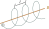
\includegraphics[scale=1.0]{figures/ch_10/fig_10_2.pdf}
		\caption[]{}
		\label{fig:10_2}
	\end{center}
	\vspace{-0.8cm}
\end{figure}

Assume that a gas is confined in a cylindrical vessel closed with a tightly fitting easily sliding piston (\fig{10_2}). If for some reason or other the gas begins to expand, it will move the piston and do work on it. The elementary work done by the gas in moving the piston through the distance $\Delta h$ is
\begin{equation*}
	\Deltap{A} = F \Delta h
\end{equation*}

\noindent
where $F$ is the force with which the gas acts on the piston. Substituting for this force the product of the gas pressure $p$ and the piston area $S$, we have
\begin{equation*}
	\Deltap{A} = p S \Delta h.
\end{equation*}

\noindent
But $S\Delta h$ is the increment of the volume of the gas $\Delta V$. Hence, the expression for the elementary work can be written as follows:
\begin{equation}\label{eq:10_10}
	\Deltap{A} = p\Delta V.
\end{equation}

The quantity $\Deltap{A}$ in \eqn{10_10} is obviously an algebraic one. Indeed, in compression of the gas, the directions of the displacement $\Delta h$ and the force $F$ with which the gas acts on the piston are opposite. Consequently, the elementary work $\Deltap{A}$ will be negative. The increment of the volume $\Delta V$ in this case will also be negative. Thus, \eqn{10_10} gives a correct expression for the work upon any changes in the volume of the gas.

If the pressure of the gas remains constant (for this to occur we must simultaneously change the temperature in the appropriate direction), the work done when the volume changes from $V_l$ to $V_2$ will be
\begin{equation}\label{eq:10_11}
	A_{12} = p(V_2 - V_1).
\end{equation}

\noindent
If a change in the volume is attended by a change in the pressure, then \eqn{10_10} holds only for sufficiently small $\Delta V$'s. In this case, the work done upon finite changes in the volume must be computed as the sum of elementary amounts of work expressed by \eqn{10_10}, \ie, by integration:
\begin{equation}\label{eq:10_12}
	A_{12} = \int_{V_1}^{V_2} p\,\deriv{V}.
\end{equation}

The expressions found for the work hold for any changes in the volume of solid, liquid, and gaseous bodies. Let us consider another example to convince ourselves that this is true. Let us take a solid body of an arbitrary shape immersed in a liquid or gaseous medium that exerts on the body the pressure $p$ identical at all points (\fig{10_3}). Assume that the body expands so that separate elementary portions of its surface $\Delta S_i$ receive different displacements $\Delta h_i$. Hence, the $i$-th portion does the work $\Deltap{A}_i$ equal to $p\Delta S_i\Delta h_i$. The work done by the body can be found as the sum of the amounts of work done by separate portions:
\begin{equation*}
	\Deltap{A} = \sum_i\Deltap{A}_i = \sum_i p \Delta S_i \Delta h_i.
\end{equation*}

\begin{figure}[t]
	\begin{center}
		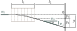
\includegraphics[scale=1.0]{figures/ch_10/fig_10_3.pdf}
		\caption[]{}
		\label{fig:10_3}
	\end{center}
	\vspace{-0.8cm}
\end{figure}

\noindent
Factoring out of the sum the value of $p$ which is identical for all the portions and noting that $\Delta S_i\Delta h_i$ gives the increment of the body's volume $\Delta V$, we can write that $\Deltap{A}=p\Delta V$, \ie, in the general case too we arrive at \eqn{10_10}.

Let us depict the process of the change in the volume of the body in a $p$-$V$ diagram (\fig{10_4}). The area of the shaded strip in the diagram corresponds to the elementary work $\Deltap{A}_i=p_i\Delta V_i$. It is obvious that the area confined between the $V$-axis, the curve $p=f(V)$, and the perpendiculars erected from points $V_1$ and $V_2$ numerically equals the work done when the volume changes from $V_1$ and $V_2$. The work done in a cyclic process numerically equals the area enclosed by the curve (\fig{10_5}). Indeed, the work on path $1$-$2$ is positive and numerically equals the the whole area under the curve, $\text{Area}_1+\text{Area}_2$ (we are considering a clockwise cycle). The work on path $2$-$1$ is negative and numerically equals the unshaded area, $\text{Area}_2$. Hence, the work during a cycle numerically equals the area enclosed by the curve (shaded area, $\text{Area}_1$). It will be positive in the direct cycle (\ie, in one conducted in the clockwise direction), and negative in the reverse cycle.

It is clear from what has been said in Sec.~\ref{sec:10_3} that the equations we have obtained may be applied only to reversible processes.

We must note that by using \eqn{10_10} (with a transition to differentials), \eqn{10_9} expressing the first law of thermodynamics can be written as follows:
\begin{equation}\label{eq:10_13}
	\derivp{Q} = \deriv{U} + p\,\deriv{V}.
\end{equation}

\begin{figure}[t]
	\begin{minipage}[t]{0.5\linewidth}
		\begin{center}
			
\includegraphics[scale=1.0]{figures/ch_10/fig_10_4.pdf}
			\caption[]{}
			\label{fig:10_4}
		\end{center}
	\end{minipage}
	\hspace{-0.0cm}
	\begin{minipage}[t]{0.5\linewidth}
		\begin{center}
			
\includegraphics[scale=1.0]{figures/ch_10/fig_10_5.pdf}
			\caption[]{}
			\label{fig:10_5}
		\end{center}
	\end{minipage}
	\vspace{-0.4cm}
\end{figure}

\section{Temperature}\label{sec:10_7}

We can arrive at a definition of the concept of temperature on the basis of the following reasoning. If contacting bodies are in a state of thermal equilibrium, \ie, do not exchange energy by heat transfer, they are said to have the same temperature. If when thermal contact is established between bodies one of them transmits energy to the other by heat transfer, then the first body is said to have a higher temperature than the second one. Many properties of bodies such as their volume and electrical resistance depend on the temperature. Any of these properties can be used for a quantitative definition of temperature.

Let us bring the body we have chosen for measuring the temperature (a thermometric body) into thermal equilibrium with melting ice. We shall assume that the body has a temperature of $0$ degrees and shall characterize quantitatively the property of the body (the temperature feature) which we intend to use for measuring the temperature. Let this feature be the volume of the body. Its value at $0$ degrees is $V_0$. Next we shall bring the same body into thermal equilibrium with water boiling under atmospheric pressure. Now we shall assume that the body in this state has a temperature of $100$ degrees, and shall determine the corresponding volume $V_{100}$. Presuming that the temperature feature we have chosen (the volume in the given example) changes linearly with the temperature, we can ascribe the following temperature to the state in which our thermometric body has the volume V:
\begin{equation}\label{eq:10_14}
	t = \frac{V - V_0}{V_{100} - V_0}\times 100\,\text{degrees}.
\end{equation}

\noindent
The temperature scale established in this way is called, as is known, the Celsius scale. An expression similar to \eqn{10_14} can also be written for the case when we use another temperature feature instead of the volume to measure the temperature.

After graduating a thermometer in this way, we can use it to measure the temperature by bringing it into thermal equilibrium with the body whose temperature we are interested in, and calculating the value of the volume.

When we compare thermometers functioning with different thermometric bodies (for example, mercury and alcohol) or different temperature features (for example, volume and electrical resistance), we find that the readings of these thermometers, which coincide at $0$ and $100$ degrees owing to their being graduated at these temperatures, do not coincide at other temperatures. It thus follows that for the unique definition of a temperature scale, in addition to the way of graduation, we must also arrive at an agreement on the choice of the thermometric body and the temperature feature. How this choice is made in establishing the so-called empirical temperature scale will be treated in the following section. Getting ahead, we shall indicate that the second law of thermodynamics can serve as the basis of a temperature scale not depending on the properties of the thermometric body (see Sec.~\ref{sec:12_3}). This scale is called the \textbf{thermodynamic temperature scale}.

The \textbf{international practical temperature scale} of 1968, formerly called the Celsius (centigrade) scale is used in engineering and for everyday purposes. Physicists find the absolute scale more convenient. The temperature $T$ measured according to this scale is related to the temperature $t$ according to the Celsius scale by the equation
\begin{equation*}
	T = t + 273.15.
\end{equation*}

\noindent
The unit of absolute temperature is the \textbf{kelvin} (\si{\kelvin}). It was previously called the degree Kelvin (\si{\degree}K). The international practical temperature is measured in \textbf{degrees Celsius} (\si{\degreeCelsius}). The sizes of the kelvin and the degree Celsius are the same. A temperature of \SI{0}{\kelvin} is referred to as \textbf{absolute zero}, and $t=\SI{-273.15}{\degreeCelsius}$ corresponds to it.

In the following (see Sec.\ref{sec:11_5}), we shall show that the absolute temperature is proportional to the mean kinetic energy of translational motion of the molecules of a substance. This is the physical meaning of absolute temperature.

\section{Equation of State of an Ideal Gas}\label{sec:10_8}

The state of a given mass of a gas is determined by the values of three parameters: the pressure $p$, volume $V$, and temperature $T$. These parameters are related to one another according to a definite law so that a change in one of them causes a change in the others. This relation can be given analytically in the form of the function
\begin{equation}\label{eq:10_15}
	F(p,V,T) = 0.
\end{equation}

An expression determining the relation between the parameters of a body is called an \textbf{equation of state} of the body. Hence, \eqn{10_15} is an equation of state of a given mass of a gas.

A gas, the interaction between whose molecules is negligibly small, has the simplest properties. Such a gas is called \textbf{ideal} (or \textbf{perfect}). The interaction between the molecules of any gas becomes negligibly small at a great rarefaction\footnote{Rarefaction here means the diminution of the density of the gas. --Ed.}, \ie, at low densities of the gas. A real gas upon sufficient rarefaction is close in its properties to an ideal one. Some gases such as air, nitrogen, and oxygen differ only slightly from an ideal gas even in usual conditions, \ie, at room temperature and atmospheric pressure. Helium and hydrogen are especially close to an ideal gas in their properties.

Gases at low densities obey the following equation with a good accuracy:
\begin{equation}\label{eq:10_16}
	\frac{pV}{T} = \text{constant}.
\end{equation}

\noindent
Consequently, this equation is an \textbf{equation of state of an ideal gas}.

According to the law established by Amadeo Avogadro (1776-1856), the moles of all gases occupy an identical volume in identical conditions (\ie, at the same temperature and pressure). In particular in the so-called \textbf{standard conditions}, \ie, at \SI{0}{\degreeCelsius} and a pressure of \SI{1}{\atm} (\SI{1.01e6}{\pascal}), the volume of a mole of any gas is $\SI{22.4}{\deci\metre\cubed\per\mole}=\SI{22.4e-3}{\metre\cubed\per\mole}$. It thus follows that when the amount of a gas is one mole, the value of the constant in \eqn{10_16} will be the same for all gases. Denoting the value of this constant corresponding to one mole by the symbol $R$, we can write \eqn{10_16} as follows:
\begin{equation}\label{eq:10_17}
	pV_{\text{m}} = RT.
\end{equation}

\noindent
We have used the subscript ``m'' with $V$ to show that we are dealing with the volume occupied by one mole of a gas at the given $p$ and $T$. Equation~\eqref{eq:10_17} is an equation of state of an ideal gas written for one mole.

The quantity $R$ is called the \textbf{molar gas constant}. According to \eqn{10_17} and Avogadro's law,
\begin{equation*}
	R = \frac{pV_{\text{m}}}{T} = \frac{\num{1.01e5}\times\num{22.4e-3}}{273}\frac{\si{\pascal}\times\si{\metre\cubed\per\mol}}{\si{\kelvin}} = \SI{8.31}{\joule\per\mole\per\kelvin}.
\end{equation*}

\noindent
For practical calculations, it is sometimes convenient to use $R$ expressed in litre-atmospheres per mole-kelvin:
\begin{equation*}
	R = \frac{\SI{1}{\atm}\times\SI{22.4}{\liter\per\mole}}{\SI{273}{\kelvin}} = \SI{0.0820}{\liter\atm\per\mole\per\kelvin}.
\end{equation*}

It is a simple matter to pass over from \eqn{10_17} for one mole to an equation for any mass $m$, taking into account that at the same pressure and temperature, $\nu$ moles of a gas will occupy a volume $\nu$ times greater than that occupied by one mole: $V=\nu V_{\text{m}}$, Multiplying \eqn{10_17} by $\nu=m/M$ (here $m$ is the mass of the gas and $M$ the mass of a mole) and introducing $V$ instead of $\nu V_{\text{m}}$, we get
\begin{equation}\label{eq:10_18}
	pV = \frac{m}{M}RT.
\end{equation}

\noindent
This equation is an equation of state of an ideal gas written for the mass $m$ of a gas.

Equation~\eqref{eq:10_18} can be given a different form. For this purpose, we shall introduce the quantity
\begin{equation}\label{eq:10_19}
	k = \frac{R}{N_{\text{A}}}
\end{equation}

\noindent
($R$ is the molar gas constant, and $N_{\text{A}}$ is the Avogadro constant). This quantity is known as the \textbf{Boltzmann constant}. It has a deeper physical meaning than the constant $R$. We shall show in Sec.~\ref{sec:11_5} that $k$ is the constant of proportionality between the mean energy of thermal motion of a molecule and the absolute temperature. Substitution of the numerical values for $R$ and $N_{\text{A}}$ in \eqn{10_19} yields
\begin{equation*}
	k = \frac{\SI{8.31}{\joule\per\mole\per\kelvin}}{\SI{6.023e23}{\per\mole}} = \SI{1.38e-23}{\joule\per\kelvin}.
\end{equation*}

Let us multiply and divide the right-hand side of \eqn{10_18} by $N_{\text{A}}$. The equation can therefore be written in the form
\begin{equation*}
	pV = \nu N_{\text{A}} k T.
\end{equation*}

\noindent
The product $\nu N_{\text{A}}$ equals the number of molecules $N$ contained in the mass $m$ of a gas. Taking this into consideration, we find that
\begin{equation}\label{eq:10_20}
	pV = NkT.
\end{equation}

Now let us divide both sides of \eqn{10_20} by $V$. Since $N/V=n$ is the number of molecules in a unit volume, we arrive at the equation
\begin{equation}\label{eq:10_21}
	p = nkT.
\end{equation}

Equations~\eqref{eq:10_18},~\eqref{eq:10_20}, and~\eqref{eq:10_21} are different forms of writing the equation of state for an ideal gas.

The ratio of the mass of a gas to the volume it occupies gives the density of the gas: $p = m/V$. According to \eqn{10_18}, the density of an ideal gas is determined by the expression
\begin{equation}\label{eq:10_22}
	\rho = \frac{M p}{R T}.
\end{equation}

\noindent
Thus, the density of an ideal gas is proportional to the pressure and inversely proportional to the temperature.

The simple relation between the temperature and the remaining parameters of an ideal gas makes it tempting to use it as a thermometric substance. Ensuring a constant volume and using the pressure of the gas as the temperature feature, we can obtain a thermometer with an ideally linear temperature scale. In the following, we shall call this scale the \textbf{ideal gas temperature scale}.

In practice, according to an international agreement, hydrogen is taken as the thermometric body. The scale established for hydrogen with the use of \eqn{10_18} is called the \textbf{empirical temperature scale}.

\section{Internal Energy and Heat Capacity of an Ideal Gas}\label{sec:10_9}

Experiments show that the internal energy of an ideal gas depends only on the temperature:
\begin{equation}\label{eq:10_23}
	U = B T.
\end{equation}

\noindent
Here $B$ is a coefficient of proportionality that remains constant within quite a broad range of temperatures.

The failure of the internal energy to depend on the volume occupied by a gas indicates that the molecules of an ideal gas do not interact with one another the overwhelming part of the time. Indeed, if the molecules did interact with one another, the internal energy would contain as an addend the potential energy of interaction, and the latter would depend on the mean distance between the molecules, \ie, on $V^{1/3}$.

It must be noted that interaction should take place upon collisions, \ie, when the molecules come very close to one another. Such collisions are very few in number in a rarefied gas, however. Each molecule spends the predominating part of its time in free flight.

\textit{The heat capacity of a body is defined as the quantity equal to the amount of heat that must be imparted to the body to raise its temperature by one kelvin}. If the amount of heat $\derivp{Q}$ imparted to a body raises its temperature by $\deriv{T}$, then its heat capacity by definition is
\begin{equation}\label{eq:10_24}
	C_{\text{body}} = \frac{\derivp{Q}}{\deriv{T}}.
\end{equation}

\noindent
This quantity is measured in joules per kelvin (\si{\joule\per\kelvin}).

We shall denote the capacity of a mole of a substance, called the \textbf{molar heat capacity}, by the symbol $C$. It is measured in joules per mole-kelvin (\si{\joule\per\mole\per\kelvin}).

The heat capacity of a unit mass of a substance is called the \textbf{specific heat capacity}. We shall use the symbol $c$ for it. The quantity $c$ is measured in joules per kilogramme-kelvin (\si{\joule\per\kilo\gram\per\kelvin}).

The following relation obviously holds between the heat capacity of a mole of a substance and the specific heat capacity of the same substance:
\begin{equation}\label{eq:10_25}
	c = \frac{C}{M}
\end{equation}

\noindent
($M$ is the molar mass).

The value of the heat capacity depends on the conditions in which a body is heated. The heat capacity for heating at a constant volume or a constant pressure is of the greatest interest. The heat capacities at constant volume and constant pressure are designated by $C_V$ and $C_p$, respectively.

When heating occurs at constant volume, a body does no work on external bodies, and, consequently, according to the first law of thermodynamics [see Eq. \eqref{eq:10_9}], all the heat is spent on the increment of the internal energy of the body:
\begin{equation}\label{eq:10_26}
	\derivp{Q}_V = \deriv{U}.
\end{equation}

\noindent
It can be seen from \eqn{10_26} that the heat capacity of any body at constant volume is
\begin{equation}\label{eq:10_27}
	C_V = \left(\diffpartial{U}{T}\right)_V.
\end{equation}

\noindent
This notation stresses the fact that when differentiating the expression for $U$ with respect to $T$, the volume must be considered constant. For an ideal gas, $U$ depends only on $T$, and \eqn{10_27} can be written in the form
\begin{equation*}
	C_V = \diff{\ab{U}{m}}{T}
\end{equation*}

\noindent
(to obtain the molar heat capacity of a gas, we must take the internal energy of a mole).

Equation~\eqref{eq:10_23} for one mole of a gas has the form $\ab{U}{m}=\ab{B}{m}T$. Differentiating it with respect to $T$, we find that $C_V=\ab{B}{m}$. Thus, the expression for the internal energy of one mole of an ideal gas can be written in the form
\begin{equation}\label{eq:10_28}
	\ab{U}{m} = C_V T
\end{equation}

\noindent
where $C_V$ is a constant quantity---the molar heat capacity of a gas at constant volume.

The internal energy of an arbitrary mass $m$ of a gas will equal the internal energy of one mole multiplied by the number of moles of the gas in the mass $m$:
\begin{equation}\label{eq:10_29}
	U = \frac{m}{M}C_V T.
\end{equation}

If a gas is heated at constant pressure, it will expand, doing positive work on external bodies. Consequently, more heat will be needed to raise the temperature of the gas by one kelvin in this case than when heating it at constant volume---part of the heat will be used by the gas to do work. Hence, the heat capacity at constant pressure must be greater than that at constant volume.

Let us write \eqn{10_13} of the first law of thermodynamics for a mole of a gas:
\begin{equation}\label{eq:10_30}
	\derivp{Q}_p = \deriv{\ab{U}{m}} + p\,\deriv{\ab{V}{m}}.
\end{equation}

\noindent
The subscript $p$ of $\derivp{Q}$ in this expression indicates that heat is imparted to the gas in conditions when $p$ is constant. Dividing \eqn{10_30} by $\deriv{T}$, we get an expression for the molar heat capacity of a gas at constant pressure:
\begin{equation}\label{eq:10_31}
	C_p = \diff{\ab{U}{m}}{T} + p\left(\diffpartial{\ab{V}{m}}{T}\right)_p.
\end{equation}

\noindent
The addend $\diffin{\ab{U}{m}}{T}$ equals, as we have seen, the molar heat capacity of a gas at constant volume. Therefore, \eqn{10_31} can be written as follows:
\begin{equation}\label{eq:10_32}
	C_p = C_v + p\left(\diffpartial{\ab{V}{m}}{T}\right)_p.
\end{equation}

The quantity $\left(\diffinpartial{\ab{V}{m}}{T}\right)_p$ is the increment of the volume of a mole when the temperature is raised by one kelvin obtained with $p$ being constant. According to the equation of state~\eqref{eq:10_17}, we have $\ab{V}{m}=RT/p$. Differentiating this expression with respect to $T$ provided that $p=\text{constant}$, we find
\begin{equation*}
	\left(\diffpartial{\ab{V}{m}}{T}\right)_p = \frac{R}{p}.
\end{equation*}

\noindent
Finally, using this result in \eqn{10_32}, we get
\begin{equation}\label{eq:10_33}
	C_p = C_v + R.
\end{equation}

Thus, the work done by a mole of an ideal gas when its temperature is raised by one kelvin at constant pressure equals the molar gas constant. It must be noted that \eqn{10_33} has been obtained by using an equation of state for an ideal gas and, consequently, holds only for an ideal gas.

The quantity
\begin{equation}\label{eq:10_34}
	\gamma = \frac{C_p}{C_V}
\end{equation}

\noindent
is a quantity characterizing every gas. For monatomic gases, its value is close to $1.67$, for biatomic gases to $1.4$, for triatomic gases to $1.33$, etc. In the following (see Sec.~\ref{sec:11_5}), we shall see that the value of $\gamma$ is determined by the number and the nature of the degrees of freedom of the molecule.

Substituting for $C_p$ in \eqn{10_34} its value from \eqn{10_33}, we have
\begin{equation*}
	\gamma = \frac{C_V + R}{C_V} = 1 + \frac{R}{C_V}
\end{equation*}

\noindent
whence
\begin{equation}\label{eq:10_35}
	C_V = \frac{R}{1 - \gamma}.
\end{equation}

\noindent
Using this value of $C_V$ in \eqn{10_29}, we get the following expression:
\begin{equation}\label{eq:10_36}
	U = \frac{m}{M}\left(\frac{RT}{\gamma - 1}\right).
\end{equation}

\noindent
Comparison with \eqn{10_18} gives still another expression for the internal energy of an ideal gas:
\begin{equation}\label{eq:10_37}
	U = \left(\frac{1}{\gamma - 1}\right) pV.
\end{equation}

\section{Equation of Adiabat of an Ideal Gas}\label{sec:10_10}

In the course of a process, a gas, in addition to an equation of state, obeys another condition determined by the nature of the process. For example, the condition $p=\text{constant}$ is observed in the so-called \textbf{isobaric process}. The condition $V=\text{constant}$ holds in an \textbf{isochoric process}. Finally, in an \textbf{isothermal process}, $T=\text{constant}$. For an ideal gas, the condition $T=\text{constant}$ is equivalent to the condition
\vspace{-12pt}
\begin{equation}\label{eq:10_38}
	pV = \text{constant}.
\end{equation}

\noindent
Equation~\eqref{eq:10_38} is called the equation of an isotherm of an ideal gas, and the curve determined by this equation is named an \textbf{isotherm}.

\textit{A process going on without heat exchange with the surroundings} is called \textbf{adiabatic}. Let us find an equation relating the parameters of an ideal gas in an adiabatic process. Introducing \eqn{10_29} for $\deriv{U}$ of an ideal gas into \eqn{10_13} of the first law of thermodynamics, we obtain
\begin{equation*}
	\derivp{Q} = \frac{m}{M}C_V\,\deriv{T} + p\,\deriv{V}.
\end{equation*}

\noindent
Since for an adiabatic process we have $\derivp{Q}=0$, the following condition must be observed:
\begin{equation}\label{eq:10_39}
	\frac{m}{M}C_V\,\deriv{T} + p\,\deriv{V} = 0.
\end{equation}

Now let us express $p$ through $V$ and $T$ in accordance with the equation of state for an ideal gas~\eqref{eq:10_18}:
\begin{equation*}
	p = \frac{m}{M}\frac{RT}{V}
\end{equation*}

\noindent
and introduce this expression into \eqn{10_39}. As a result, after cancelling the factor $m/M$ differing from zero, we get
\begin{equation*}
	C_V\,\deriv{T} + RT\,\frac{\deriv{V}}{V} = 0.
\end{equation*}

\noindent
Let us transform the above expression as follows:
\begin{equation*}
	\frac{\deriv{T}}{T} + \frac{R}{C_V}\,\frac{\deriv{V}}{V} = 0.
\end{equation*}

\noindent
This expression can be written in the form
\begin{equation*}
	\upd\left(\ln{T} + \frac{R}{C_V}\,\ln{V}\right) = 0
\end{equation*}

\noindent
whence it follows that in an adiabatic process
\begin{equation}\label{eq:10_40}
	\ln{T} + \frac{R}{C_V}\,\ln{V} = \text{constant}.
\end{equation}

In accordance with \eqn{10_35}, the ratio $R/C_V$ can be replaced withy $\gamma - 1$, where $\gamma=C_p/C_V$. Making this substitution in \eqn{10_40} and converting to a power, we get
\begin{equation}\label{eq:10_41}
	T V^{\gamma - 1} = \text{constant}.
\end{equation}

This equation is an equation of an adiabat of an ideal gas in variable $T$ and $V$. We can pass over from this equation to one in variable $p$ and $V$ by replacing $T$ in it with $p$ and $V$ in accordance with the equation of state for an ideal gas~\eqref{eq:10_18}:
\begin{equation*}
	T = \frac{M}{m}\frac{pV}{R}.
\end{equation*}

\noindent
Using this expression in \eqn{10_41} and taking into account that $m$, $M$ and $R$ are constants, we get
\begin{equation}\label{eq:10_42}
	p V^{\gamma} = \text{constant}.
\end{equation}

\noindent
[The values of the constants in Eqs.~\eqref{eq:10_40}-\eqref{eq:10_42} are obviously
different.]

Expression~\eqref{eq:10_42} is an equation of an adiabat of an ideal gas in variable $p$ and $V$. It is also called the \textbf{Poisson equation}.

\begin{figure}[t]
	\begin{center}
		
\includegraphics[scale=1.0]{figures/ch_10/fig_10_6.pdf}
		\caption[]{}
		\label{fig:10_6}
	\end{center}
	\vspace{-0.8cm}
\end{figure}

It follows from a comparison of the adiabat equation~\eqref{eq:10_42} with the isotherm equation~\eqref{eq:10_38} that an adiabat is steeper than an isotherm. Let us calculate $\diffin{p}{V}$ for an isotherm and an adiabat at the same point with the coordinates $p$ and $V$ (\fig{10_6}). Differentiation of \eqn{10_38} yields
\begin{equation*}
	p\,\deriv{V} + V\,\deriv{p} = 0
\end{equation*}

\noindent
whence for an isotherm we obtain
\begin{equation}\label{eq:10_43}
	\diff{p}{V} = -\frac{p}{V}.
\end{equation}

\noindent
Differentiation of Eq. (10.42) yields
\begin{equation*}
	p \gamma V^{\gamma - 1}\,\deriv{V} + V^{\gamma}\,\deriv{p} = 0
\end{equation*}

\noindent
whence
\begin{equation*}
	\diff{p}{V} = -\gamma \frac{p}{V}.
\end{equation*}

\noindent
Thus, the slope of an adiabat is $\gamma$ times greater than that of an isotherm.

We assumed in all our reasoning that the state of a gas at each moment is characterized by definite values of the parameters $p$ and $T$, \ie, in other words, that the adiabatic process being considered is reversible. We know that only a very slow process can be reversible. At the same time, since nature knows of no substances that do not conduct heat absolutely, the amount of heat exchanged by a system with its surroundings will be the smaller, the shorter is the time taken by a process.

Thus, only fast processes can be close to an adiabatic one. An example of such a process are the compression and expansion occurring at each point of a gas in which a sound wave is propagating. Notwithstanding the fact that within the confines of a large volume the state of the gas is not an equilibrium one ($p$ and $T$ are different at different points), the behaviour of the gas within the limits of each sufficiently small volume is quite satisfactorily described by \eqn{10_42} of an adiabat.

\section{Polytropic Processes}\label{sec:10_11}

\textit{Processes in which the heat capacity of a body remains constant} are defined as \textbf{polytropic} ones. Thus, the condition which is observed in a polytropic process is
\begin{equation}\label{eq:10_44}
	C = \text{constant}.
\end{equation}

Let us find the equation of a polytrope for an ideal gas. We shall write equation~\eqref{eq:10_13} of the first law for one mole of gas, substituting $C\,\deriv{T}$ for $\derivp{Q}$ and $C_V\,\deriv{T}$ for $\deriv{U}$:
\begin{equation}\label{eq:10_45}
	C\,\deriv{T} = C_V\,\deriv{T} + p\,\deriv{V}.
\end{equation}

\noindent
This equation includes all three parameters: $p$, $V$ and $T$. One of them can be excluded with the aid of an equation of state. To obtain an equation of a polytrope directly in variable $p$ and $V$, let us exclude $T$. For this end, let us differentiate the equation $pV=RT$:
\begin{equation}\label{eq:10_46}
	p\,\deriv{V} + V\,\deriv{p} = R\,\deriv{T} + .
\end{equation}

\noindent
Excluding $\deriv{T}$ from Eqs.~\eqref{eq:10_45} and~\eqref{eq:10_46} and bringing together similar terms, we get
\begin{equation}\label{eq:10_47}
	(C - C_V - R) p\,\deriv{V} + (C - C_V) V\,\deriv{p} = 0.
\end{equation}

\noindent
Substituting $C_p$ for $C_V+R$ [see \eqn{10_33}] and dividing \eqn{10_47} by $pV$, we arrive at the differential equation
\begin{equation}\label{eq:10_48}
	(C - C_p)\,\frac{\deriv{V}}{V} + (C - C_V) \,\frac{\deriv{p}}{p} = 0.
\end{equation}

The quantities $C$, $C_p$, and $C_V$ are constants. Therefore, integration of \eqn{10_48} gives the expression
\begin{equation}\label{eq:10_49}
	(C - C_p)\,\ln{V} + (C - C_V)\,\ln{p} = \text{constant}.
\end{equation}

\noindent
Dividing this expression by $C-C_V$ (which is possible if $C\neq C_v$) and converting to a power, we get
\begin{equation}\label{eq:10_50}
	pV^n = \text{constant}
\end{equation}

\noindent
where
\begin{equation}\label{eq:10_51}
	n = \frac{C - C_p}{C - C_V}.
\end{equation}

It is exactly \eqn{10_50} that is the required equation of a polytrope of an ideal gas for $C\neq C_v$. The quantity $n$ determined by \eqn{10_51} is called the \textbf{polytropic exponent} or \textbf{index}.

Let us turn to \eqn{10_49} to establish the nature of a polytropic process when $C=C_V$. For this condition, the equation acquires the form $(C-C_p)\ln{V}=\text{constant}$, whence it follows that $V$ in the course of the process remains constant. Hence, a polytropic process with $C=C_V$ is an isochoric one. This could be foreseen because $C_V=\text{constant}$ and is the heat capacity at constant volume, \ie, in	an isochoric process. By \eqn{10_51}, the polytropic exponent in an isochoric process equals infinity.

The other processes treated in the preceding section also relate to the category of polytropic processes. For an isobaric process, we have $n=0$ [see \eqn{10_50}], for an isothermal one $n=1$, and, finally, for an adiabatic process $n=\gamma$. The value of the polytropic exponent $n$ for these processes are given in Table~\ref{table:10_1}.

\begin{table}[!b]
	\renewcommand{\arraystretch}{1.2}
	\caption{ }
	\vspace{-0.6cm}
	\label{table:10_1}
	\begin{center}\resizebox{0.233\linewidth}{!}{
			\begin{tabular}{lc}
				\toprule[1pt]
				\textbf{Process} & $n$\\
				\midrule[0.5pt]\midrule[0.5pt]
				Isobaric & 0\\
				Isothermal & 1\\
				Adiabatic & $\gamma$\\
				Isochoric & $\infty$\\
				\bottomrule[1pt]
			\end{tabular}
	}\end{center}
\end{table}

Solving \eqn{10_51} relative to $C$, we get an equation for the heat capacity of an ideal gas in a polytropic process:
\begin{equation}\label{eq:10_52}
	C = \frac{n C_V - C_p}{n - 1}.
\end{equation}

\noindent
The introduction of $n=\gamma$ causes \eqn{10_52} to become equal to zero [\eqn{10_35} must be taken into account in verifying this statement]. Consequently, the heat capacity of an ideal gas in an adiabatic process equals zero. The heat capacity of all bodies vanishes in an adiabatic process. This can be seen from the fact that in an adiabatic process $\derivp{Q}=0$, whereas $\deriv{T}$ differs from zero.

The introduction of $n=1$ causes \eqn{10_52} to equal infinity. Thus, in an isothermal process, the heat capacity is infinitely great. The explanation is that in an isothermal process $\deriv{T}=0$, whereas $\derivp{Q}$ differs from zero.

\section{Work of an Ideal Gas in Different Processes}\label{sec:10_12}

The work done by a body on external bodies when it passes from state $1$ to state $2$ is
\begin{equation}\label{eq:10_53}
	A_{12} = \int_{V_1}^{V_2} p\,\deriv{V}
\end{equation}

\noindent
[see \eqn{10_12}]. To perform integration, we must express $p$ through $V$. For this purpose, we shall use the relation between $p$ and $V$ in different processes.

Equation~\eqref{eq:10_50} of a polytrope of an ideal gas can be written as follows:
\begin{equation*}
	pV^n = p_1V_1^n = p_2V_2^n
\end{equation*}

\noindent
where $ p_1, V_1$ and $ p_2, V_2$ are the values of the pressure and volume of the gas in the first (initial) and second (final) states, respectively, and $p$ and $V$ are the pressure and volume in any intermediate state. The above equation allows us to express the pressure of a gas through its volume and the values of the parameters in the initial or final state. Taking the former, we have
\begin{equation*}
	p = \frac{p_1V_1^n}{V^n}.
\end{equation*}

\noindent
Introduction of this equation into \eqn{10_53} yields
\begin{equation}\label{eq:10_54}
	A_{12} = p_1 V_1^n\, \int_{V_1}^{V_2} \frac{\deriv{V}}{V^n}.
\end{equation}

\noindent
Let us first consider the case when $n\neq 1$; the integral in \eqn{10_54} for it is
\begin{equation*}
	\int_{V_1}^{V_2} \frac{\deriv{V}}{V^n} = \left(\frac{1}{n-1}\right) \left(\frac{1}{V_1^{n-1}} - \frac{1}{V_2^{n-1}}\right).
\end{equation*}

\noindent
Using this value of the integral in \eqn{10_54} and performing simple transformations, we get
\begin{equation}\label{eq:10_55}
	A_{12} = \frac{p_1 V_1}{n-1} \left[1 - \left(\frac{V_1}{V_2}\right)^{n-1} \right].
\end{equation}

This equation can be transformed by taking advantage of the fact that no matter what process occurs with an ideal gas, its parameters are related by an equation of state. In particular, this also holds for the initial state:
\begin{equation}\label{eq:10_56}
	p_1 V_1 = \frac{m}{M}RT_1.
\end{equation}

\noindent
Taking \eqn{10_56} into account, we can write \eqn{10_55} in the form
\begin{equation}\label{eq:10_57}
	A_{12} = \frac{m}{M} \left(\frac{RT_1}{n-1}\right) \left[1 - \left(\frac{V_1}{V_2}\right)^{n-1} \right].
\end{equation}

Equations~\eqref{eq:10_55} and~\eqref{eq:10_57} give the work done by an ideal gas in any polytropic process except for an isothermal one [which corresponds to $n=1$. In this case, Eqs.~\eqref{eq:10_55} and~\eqref{eq:10_57} become indefinite]. In particular, for an adiabatic process
\begin{equation}\label{eq:10_58}
	A_{12} = \left(\frac{p_1 V_1}{\gamma - 1}\right) \left[1 - \left(\frac{V_1}{V_2}\right)^{n-1} \right]
\end{equation}

\noindent
or
\begin{equation}\label{eq:10_59}
	A_{12} = \frac{m}{M} \left(\frac{RT_1}{\gamma - 1}\right) \left[1 - \left(\frac{V_1}{V_2}\right)^{n-1} \right].
\end{equation}

To calculate the work of an ideal gas in an isothermal process, let us express the pressure in \eqn{10_53} through other quantities in accordance with an equation of state. The result is (we can put $T$ outside the integral since it is constant):
\begin{equation*}
	A_{12} = \frac{m}{M}RT\, \int_{V_1}^{V_2} \frac{\deriv{V}}{V} = \frac{m}{M} RT\,\ln\left(\frac{V_2}{V_1}\right).
\end{equation*}

\noindent
Thus, the work done by an ideal gas in an isothermal process is
\begin{equation}\label{eq:10_60}
	A_{12} = \frac{m}{M} RT\,\ln\left(\frac{V_2}{V_1}\right).
\end{equation}

In an isobaric process, the work done by any body including an ideal gas, as can be seen from \eqn{10_53}, is
\begin{equation}\label{eq:10_61}
	A_{12} = p(V_2 - V_1).
\end{equation}

\noindent
The same result is obtained if we assume that $n=0$ in \eqn{10_55}. We shall note in concluding that the work equals zero in an isochoric process. This holds for any bodies.

\section{Van der Waals Gas}\label{sec:10_13}

We mentioned in Sec.~\ref{sec:10_8} that the behaviour of real gases is well described by \eqn{10_17}, \ie,
\begin{equation*}
	p\ab{V}{m} = RT
\end{equation*}

\noindent
only at low densities, \ie, at not too high pressures and sufficiently high temperatures [see \eqn{10_22}]. Considerable deviations from this equation are observed with an increase in the pressure and a decrease in the temperature. The second column of Table~\ref{table:10_2} gives the values of the product $pV$ for the mass of nitrogen occupying a volume of one litre in standard conditions. These values are given for different pressures and the same temperature \SI{0}{\degreeCelsius}.

\begin{table}[!b]
	\vspace{-0.2cm}
	\renewcommand{\arraystretch}{1.2}
	\caption{ }
	\vspace{-0.6cm}
	\label{table:10_2}
	\begin{center}\resizebox{0.6\linewidth}{!}{
			\begin{tabular}{ccc}
				\toprule[1pt]
				$p$, [\si{\atm}] & $pV$, [\si{\atm\liter}] & $\left(p+\dfrac{a'}{V^2}\right)(V-b')$, [\si{\atm\liter}]\\
				\midrule[0.5pt]\midrule[0.5pt]
				$1$ 	& 	$1.000$ 	&	$1.000$\\
				$100$ 	&	$0.994$		&	$1.000$\\
				$200$	&	$1.048$		&	$1.009$\\
				$500$	&	$1.390$		&	$1.014$\\
				$1000$	&	$2.069$		&	$0.893$\\
				\bottomrule[1pt]
			\end{tabular}
	}\end{center}
\end{table}

According to \eqn{10_17}, the product $pV$ must remain constant when the temperature does not change. Actually, as can be seen from the table, appreciable deviations are observed at a pressure of about \SI{200}{\atm}. They grow continuously with increasing pressure and reach over $100$\% at \SI{1000}{\atm}. These deviations are not surprising because when the density grows, the volume of the molecules and the interaction between them begin to play a greater and greater part.

A great variety of equations were proposed to describe the behaviour of gases within a broad density range. The one proposed by J. van der Waals is the simplest of them, while giving sufficiently good results. This equation was obtained by introducing corrections into \eqn{10_17} and has the following form:
\begin{equation}\label{eq:10_62}
	\left(p+\frac{a}{\ab{V}{m}^2}\right)(\ab{V}{m} - b) = RT
\end{equation}

\noindent
where $p$ is the pressure exerted on the gas from outside (equal to the pressure of the gas on the walls of the vessel it occupies), and $a$ and $b$ are van der Waals constants. Their values differ for different gases and are determined experimentally. If the pressure is measured in pascals and the volume in cubic metres per mole, then the constant $a$ is in \si{\pascal~\metre^6~\mole^{-1}}, and the constant $b$ is in \si{\metre\cubed\per\mole}. Sometimes the constants $a$ and $b$ are expressed in \si{\atm\liter\squared} and \si{\liter\per\mole}, respectively.

Owing to the mutual attraction between its molecules, a gas, as it were, is compressed by a greater pressure than the pressure $p$ exerted on it by the walls of the vessel confining it. The correction $a/\ab{V}{m}^2$ characterizes the addition to the external pressure due to the mutual attraction of the molecules. Molecules have an appreciable action on one another within the limits of small distances called the \textbf{radius of molecular action}. The force of mutual attraction of two elementary volumes having dimensions of the order of this radius is proportional both to the number of molecules contained in one of the volumes and to that in the other volume. Each of these numbers, in turn, is proportional to the number of molecules in unit volume, \ie, is inversely proportional to the volume of the gas. These considerations can be used to explain the circumstance that the correction to the pressure in \eqn{10_62} has the form $a/\ab{V}{m}^2$.

Since the molecules have a finite volume, the space available for motion of the molecules is less than the volume of the vessel $\ab{V}{m}$ The correction $b$ in \eqn{10_62} characterizes the part of the volume that is not available for motion of the molecules. In its order of magnitude, it equals several total volumes of the molecules contained in a mole of a gas.

Equation~\eqref{eq:10_62} has been written for one mole of a gas. To go over to an equation for an arbitrary mass $m$, we must take into account that $\nu$ moles of a gas in the same conditions occupy a volume that is $\nu$ times greater: $V=\nu\ab{V}{m}.$ Substituting $V/\nu$ for $\ab{V}{m}$ in \eqn{10_62}, we get
\begin{equation*}
	\left(p + \frac{\nu^2 a}{V^2}\right) \left(\frac{V}{\nu} - b\right) = RT.
\end{equation*}

\noindent
Multiplying this equation by $\nu$ and introducing the symbols
\begin{equation}\label{eq:10_63}
	a' = \nu^2 a,\quad b' = \nu b
\end{equation}

\noindent
we arrive at the van der Waals equation for $\nu$ moles:
\begin{equation}\label{eq:10_64}
	\left(p + \frac{a'}{V^2}\right) (V - b') = \nu RT.
\end{equation}

\noindent
The symbols $a'$ and $b'$ designate the van der Waals constants for $\nu$ moles. Equations~\eqref{eq:10_63} show how they are related to $a$ and $b$. The constant $a'$ is measured in \si{\pascal~\metre^6}, and $b'$ in \si{\metre\cubed}.

How much better the van der Waals equation shows the behaviour of gases than \eqn{10_17} can be seen from the data contained in Table~\ref{table:10_2}. The third column of the table gives the values of the quantity $(p+a'/V^2)(V-b')$, which ought to be constant according to \eqn{10_64}, for the same mass of nitrogen for which the values of $pV$ are given in the second column. Inspection of the table shows that the van der Waals equation agrees much better with experimental data than \eqn{10_17}.

Since all real gases approach ideal gases in their properties when their density diminishes, the van der Waals equation in the limit, when the volume tends to infinity, transforms into \eqn{10_17}. We can convince ourselves that this is true by factoring out $p$ and $V$ in \eqn{10_64}:
\begin{equation*}
	pV\left(1 + \frac{1}{pV}\frac{a'}{V}\right)\left(1 - \frac{b'}{V}\right) = \nu RT
\end{equation*}

\noindent
and taking into consideration that the product $pV$ is approximately constant.

Real gases obey the van der Waals equation only approximately. An imaginary gas that obeys \eqn{10_62} exactly is called a van der Waals gas.

The internal energy of a van der Waals gas must include, in addition to the kinetic energy of the molecules, the energy of interaction between them. To find the internal energy of a van der Waals gas, let us take advantage of the circumstance that the work done in the expansion of a gas against the forces of mutual attraction of the molecules to one another equals the increment of the interaction energy: $\derivp{A}= \deriv{\ab{E}{p}}$. The forces of mutual attraction between the molecules are taken into account in \eqn{10_62} with the aid of the addition $a/\ab{V}{m}^2$ to the pressure. Accordingly, the work against the forces of interaction between the molecules can be represented in the form $(a/\ab{V}{m}^2)\,\deriv{\ab{V}{m}}$ (similarly, the work done by a gas against the external forces is determined by the expression $p\,\deriv{V}$). Thus,
\begin{equation*}
	\deriv{\ab{E}{p}} = \frac{a}{\ab{V}{m}^2}\,\deriv{\ab{V}{m}}.
\end{equation*}

\noindent
Integration of this expression shows that
\begin{equation}\label{eq:10_65}
	\ab{E}{p} = -\frac{a}{\ab{V}{m}} + \text{constant}.
\end{equation}

The internal energy of a van der Waals gas depends on both the volume and the temperature. Hence, the expression for $U$ has the form
\begin{equation*}
	U = f(T) - \frac{a}{\ab{V}{m}}
\end{equation*}

\noindent
[we have included the constant of \eqn{10_65} in $f(T)$]. This expression in the limit, when the volume tends to infinity, must transform into \eqn{10_28} for the internal energy of an ideal gas. Therefore, $f(T)=C_VT$.

Thus, the internal energy of a mole of a van der Waals gas is determined by the equation
\begin{equation}\label{eq:10_66}
	\ab{U}{m} = C_VT - \frac{a}{\ab{V}{m}}.
\end{equation}

\noindent
The internal energy of $\nu$ moles will be $\nu$ times greater:
\begin{equation}\label{eq:10_67}
	U = \nu C_VT - \frac{a'}{V}
\end{equation}

\noindent
(we have taken into consideration that $\nu^2a=a'$ and $\nu\ab{V}{m}=V$). By Eqs.~\eqref{eq:10_66} and~\eqref{eq:10_67}, we can find the approximate values of the internal energy of real gases.

\section{The Barometric Formula}\label{sec:10_14}

The atmospheric pressure at the altitude $h$ is due to the weight of the layers of gas above this altitude. Let $p$ be the pressure at the altitude $h$. Hence, the pressure at the altitude $h+\deriv{h}$ will be $p+\deriv{p}$. If $\deriv{h}$ is greater than zero, then $\deriv{p}$ will be less than zero because the weight of the higher layers of the atmosphere and, therefore, the pressure, diminish with the altitude. The difference between the pressures $p$ and $p+\deriv{p}$ equals the weight of the gas contained in the volume of a cylinder with a base area of unity and an altitude of $\deriv{h}$ (\fig{10_7}):
\begin{equation*}
	p - (p + \deriv{p}) = \rho g\,\deriv{h}
\end{equation*}

\noindent
where $\rho$ is the density of the gas at the altitude $h$. Hence,
\begin{equation}\label{eq:10_68}
	\deriv{p} = -\rho g\,\deriv{h}.
\end{equation}

\begin{figure}[t]
	\begin{minipage}[t]{0.4\linewidth}
		\begin{center}
			
\includegraphics[scale=1.0]{figures/ch_10/fig_10_7.pdf}
			\caption[]{}
			\label{fig:10_7}
		\end{center}
	\end{minipage}
	\hspace{-0.05cm}
	\begin{minipage}[t]{0.5\linewidth}
		\begin{center}
			
\includegraphics[scale=1.0]{figures/ch_10/fig_10_8.pdf}
			\caption[]{}
			\label{fig:10_8}
		\end{center}
	\end{minipage}
	\vspace{-0.4cm}
\end{figure}

We indicated in Sec.~\ref{sec:10_8} that air differs only slightly from an ideal gas in its behaviour in conditions close to standard ones. Therefore, the density of air can be calculated by \eqn{10_22}. The introduction of this equation into \eqn{10_68} yields
\vspace{-12pt}
\begin{equation}\label{eq:10_69}
	\deriv{p} = -\frac{Mpg}{RT}\,\deriv{h}.
\end{equation}

\noindent
The quantity $M$ in this equation numerically equals the average molecular mass of air determined with account taken of the content of nitrogen, oxygen, and other gases in it. It can be seen from \eqn{10_69} that
\begin{equation}\label{eq:10_70}
	\frac{\deriv{p}}{p} = -\frac{Mg}{RT}\,\deriv{h}.
\end{equation}

\noindent
The temperature $T$ is a function of $h$. If we know the form of this function, we can integrate \eqn{10_70} and find how $p$ depends on $h$. For a constant temperature, \ie, for an isothermal atmosphere, integration of \eqn{10_70} leads to the expression
\begin{equation*}
	\ln({p} = -\frac{Mgh}{RT} + \ln{C}
\end{equation*}

\noindent
where $C$ is a constant (it is convenient here to denote the integration constant by $\ln{C}$). Raising this expression to a power yields
\begin{equation*}
	p = C\,\exp\left(- \frac{Mgh}{RT} \right).
\end{equation*}

\noindent
Introducing $h=0$ into this expression, we find that $C=p_0$, where $p_0$ is the pressure at the altitude $h=0$.

Thus, for our assumption on constancy of the temperature, the dependence of the pressure on the altitude is given by the formula
\begin{equation}\label{eq:10_71}
	p = p_0\,\exp\left(- \frac{Mgh}{RT} \right).
\end{equation}

\noindent
This is the \textbf{barometric formula}. A glance at it shows that the pressure diminishes with the altitude the more rapidly, the heavier is the gas (the greater is $M$) and the lower is the temperature. Figure~\ref{fig:10_8} shows two curves corresponding to \eqn{10_71}. They can be interpreted either as corresponding to different $M$'s (at the same temperature), or to different $T$'s (at the same values of $M$).
